\documentclass[12pt,a4paper]{article}
%\DeclareMathSizes{12}{14}{10}{6}
\usepackage[utf8]{inputenc}
\usepackage[T1]{fontenc}
\usepackage[english]{babel}
\usepackage[outer=25mm,inner=35mm,top=25mm,bottom=25mm]{geometry}

\usepackage{indentfirst}
\usepackage{colortbl}
\usepackage{amsmath}
\usepackage{caption}
\usepackage{graphicx}
\usepackage{setspace}
\usepackage{hyperref}
\usepackage[export]{adjustbox}
\usepackage{listings}
\usepackage{wrapfig}
\usepackage{float}
\usepackage[
backend=biber,
natbib=true,
style=mla,
sorting=nyt
]{biblatex}

\addbibresource{ref.bib}


\frenchspacing
\linespread{1.5}


\begin{document}
	\begin{center}
		\section*{TSA - Empirical project: Could interest rate hikes burst the housing bubble?}
		Péter Horváth	
	\end{center}
\section*{Abstract}
In this paper I will be analyzing the US housing market from a monetary policy point of view. In the recent years we saw a vast increase in real housing prices, which could possibly have come to pass due to the low interest rate environment. Recent economic developments causing heightened inflationary pressure however lead most central banks to start an aggressive interest rate rise policy, ending the low interest rate era. This leads us to the proposed question - could the interest rate hikes burst the housing bubble? To investigate this, I will estimate a two-regime TVAR model dependent on housing prices using US data. Results will show that although the size of the impact of an interest rate shock  in both regimes, its persistence much stronger when housing prices are high.



\pagebreak

\section{Introduction}
Over the recent years, studying the relationship between the housing market and the economy has been gaining traction, as it provides key implications for conducting appropriate policy making in the fields of fiscal, macroprudential and monetary authorities. \textcolor{blue}{\cite{iacoviello2007}} use Bayesian DSGE methods to show that housing shocks have a non-negligible spillover effect on the economy as they influence consumption decisions. \textcolor{blue}{\cite{schiller2003}}'s paper although published almost two decades ago, show using survey data, that there was strong evidence of housing being a bubble - a statement that is likely true in current times as well. \textcolor{blue}{\cite{dsgemacroprud}} point to the importance of understanding the underlying shocks to the housing market for conducting optimal monetary and macroprudential policies also using a DSGE model.\\

\noindent Based on the recent years’ development in the housing market and monetary policy trends, some intriguing questions arise, such as ‘Is the housing market a bubble?’, ‘Could the large-scale monetary easing programs have contributed to the creation of it?’ and most recently ‘Could the sharp monetary tightening cause the housing market to crash?’.  In this paper, I will be seeking answers to the latter question. I hypothesize that tightening monetary conditions when the housing market is heated, could cause it to crash, i.e. interest rate hikes have a significantly larger impact on housing prices when they are high. This assumes a non-linear relationship between the economy and the housing market. For this reason, I believe that using a non-linear Threshold Vector-Autoregressive model (TVAR) could be appropriate to implement.\\  

\noindent The rest of the paper will be outlined as follows. In section (2) I will give a brief description of the data used for estimation purposes and describe the empirical strategy in detail. Section (3) reports the results of the estimation, and section (4) concludes.

\section{Data and empirical strategy}
For the purposes of this analysis I will be relying on quarterly data from the US, ranging from January 1973 to December 2021. House prices will be measured by the real residential property price index and the impact of monetary policy shocks will be identified by shocks to the Federal Funds Rate. As the credit channel of monetary policy is rather important for the housing market, the inclusion of variables that represent the housing loan market is necessary as well. For this purpose I will be including the volume of real estate loans from all banks and the 30-year fixed rate mortgage average as interest rate paid on housing loans. To further enrich the model, I will add quarterly GDP as a measure of economic activity. All data used are retrieved from the Federal Reserve Economic Database.
 \begin{center}
	\begin{figure}[h!]
			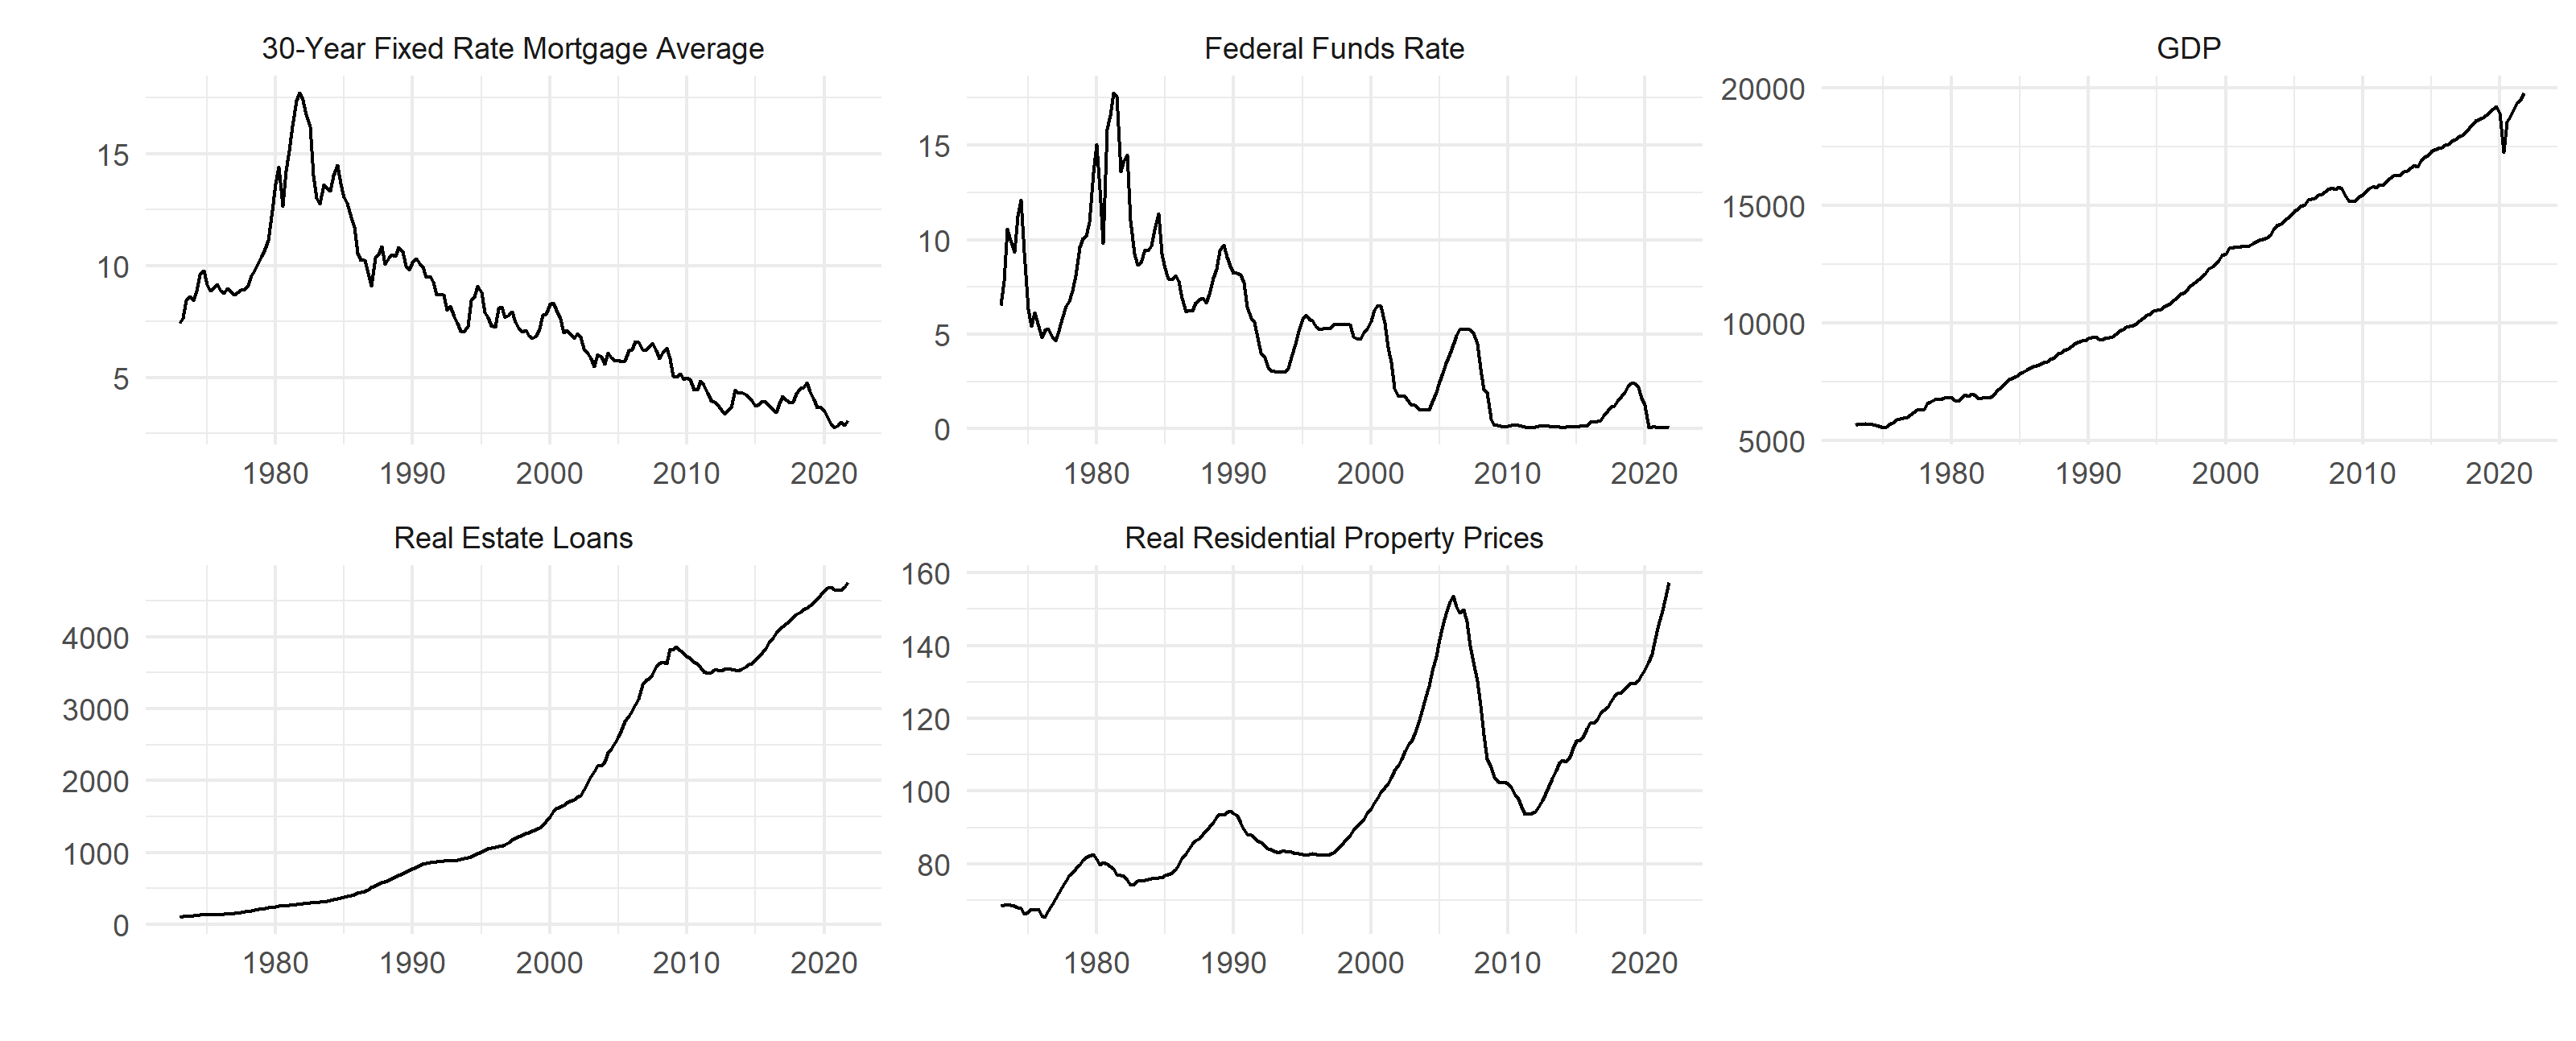
\includegraphics[width = \textwidth]{dataplot.png}
			\caption{Time series plots of data series used in levels}
	\end{figure}
\end{center}
Even without running stationarity tests, we can see that neither of the above variables are stationary. For this reason, in order to make the estimated model more stable I will be including GDP, housing loan volume and the residential property price index using log-differences, however I will leave the interest rates in as levels. I believe this combination will give a model with enough stability and clear economic interpretation (as log-differenced variables can be interpreted as growth rates). Another possibility could be to check for cointegrating relationships between these variables and use a VECM model instead of a VAR á la \textcolor{blue}{\cite{iacoviello2008credit}}, however this is beyond the scope of this paper.\\

To study the relationship between monetary policy shocks and house prices, as mentioned before, I believe fitting a vector-autoregressive model seems appropriate. First, let's consider a simple VAR model which can be written in a recursive formula such as
\begin{equation}
	B(L)Y_{t} = \alpha_{0} + \epsilon_{t},
\end{equation}
where  $B(L)$ is the matrix of coefficients at lag L, $Y_{t}$ is the vector of endogenous variables, $\alpha_{0}$ is the vector of constants and $\epsilon_{t}$ is the error term.\\
An adequate way to analyze the impact of a monetary policy shock is to identify structural shocks and impose a set of restrictions on the model. For this purpose I will be using choleski decomposition to a lower-triangular matrix, therefore ordering the variables
\begin{equation}
	Y_{t} = 
	\begin{Bmatrix}
		FFR_{t} \\
		M30_{t} \\
		HLOAN_{t} \\
		GDP_{t} \\
		HPRICE_{t}
	\end{Bmatrix}
\end{equation}
where $FFR_{t}$ is the Federal Funds Rate, $M30_{t}$ is the 30-year fixed rate mortgage average, $HLOAN_{t}$ is the quarterly growth in housing loan volume, $GDP_{t}$ is the quarterly GDP growth, and $HPRICE_{t}$ is the quarterly growth in real residential prices. The ordering is set up assuming the FFR to be the most exogenous - as it is determined by the Federal Reserve bank. Changes in the FFR would drive the fluctuations in  loan market by directly impacting the mortgage rate and thus driving the growth in loans taken up. The credit and interest rate channel would impact economic activity would have a transmission effect on economic activity as measured by GDP growth, and both the credit channel and economic outlook would impact fluctuations of housing prices. From this simple structural VAR model we would get the following impulse responses for a 1 percentage point shock to the interest rate \footnote{Lag order of 1 selected by the Schwarz-Bayesian Information Criterion}:
 \begin{center}
	\begin{figure}[h!]
		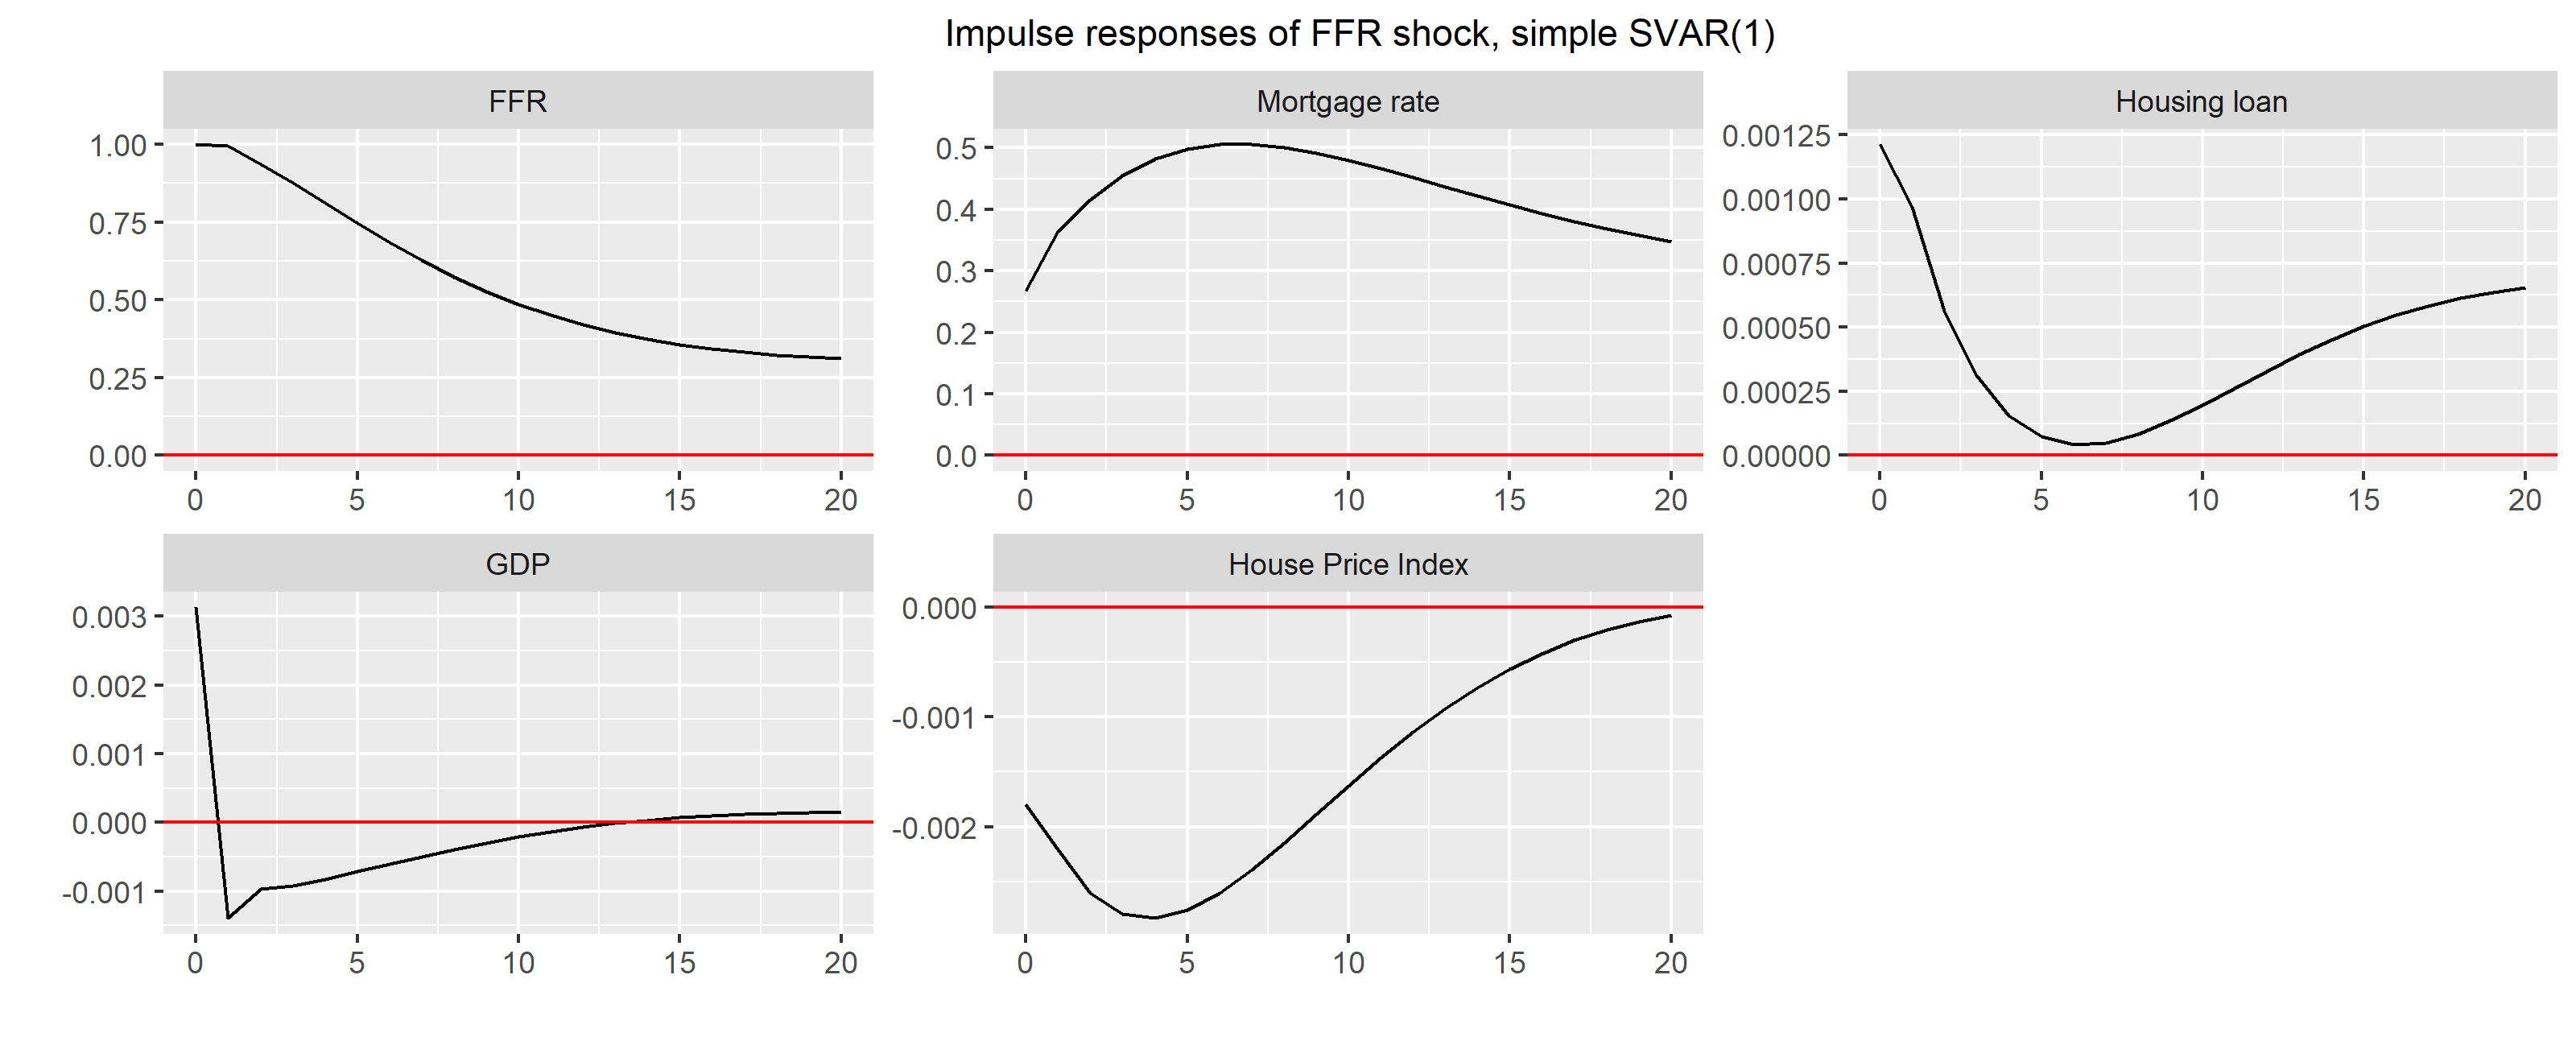
\includegraphics[width = \textwidth]{svarirf.png}
		\caption{Impulse responses of a 1 percentage point interest rate rise in a SVAR(1) model}
	\end{figure}
\end{center}
From this we see that on impact, the mortgage rate rises by roughly a third, 30 basis points, and continue a sluggish persistent rise before starting to decay. Economic activity rises sharply, but drops to contraction roughly a quarter after impact, and recovers quickly. This could be explained by the Federal Reserve raising interest rates when the economy is overheated, and the monetary transmission mechanism having a lagged impact on the economy. An interesting result is the rise in loan volume on impact. An explanation could be the drop in property prices, incentivizing investors to increase their activity in the real estate market. However, as the mortgage rate stays persistently high, while housing prices take several quarters to rebound, the growth in loan volume dampens, only to rebound later as mortgage rates decrease, and housing prices show a steady rebound.\\

\noindent I find this explanation somewhat unsatisfactory however. Would housing loans show an upward slope if housing prices were growing at a lower rate (or perhaps were decreasing in the first place)? Could housing prices drop more sharply if they were higher to begin with? Could there be a boom-bust cycle relationship, where the interest rate shocks are perhaps more persistent? \textcolor{blue}{\cite{jarocinski2008house}} and \textcolor{blue}{\cite{musso2011housing}} both study the relationship between housing prices using SVAR models and hint at the possibility of there being a nonlinear relationship. \textcolor{blue}{\cite{ahamada2013retrospective}}, \textcolor{blue}{\cite{ghodsi2017nonlinear}} and \textcolor{blue}{\cite{kang2014non}} all suggest a non-linear relationship between housing prices and the economy. To provide further evidence, I conducted a bootstrapped multivariate version of the \textcolor{blue}{\cite{hansen1999testing}}  likelihood-ratio test as proposed by \textcolor{blue}{\cite{lo2001threshold}} using the algorithm implemented by \textcolor{blue}{\cite{stigler2019}}. 
 \begin{center}
	\begin{figure}[h!]
		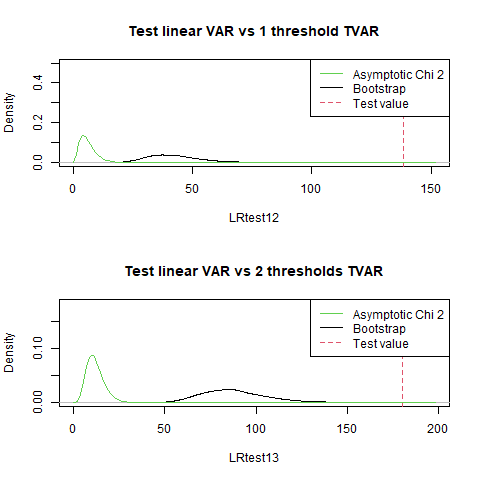
\includegraphics[width = 0.75\textwidth]{tvartest.png}
		\caption{Bootstrapped LR test for non-linearity}
	\end{figure}
\end{center}
As seen in Figure 3 above, testing a linear VAR vs either a two-threshold or three-threshold variant results in a close to zero p-value, thus rejecting the linear model over any of the non-linear variants. For the purposes of this paper, the two-threshold variant should suffice, thus we can formulate our model as: 
 \begin{equation}
 	Y_{t} = \Theta_{1}I(X_{t-1})Y_{t-1}+\Theta_{2}I(X_{t-1})Y_{t-1} + \epsilon_{t},
 \end{equation}
where - as before - $Y_{t}$ is the list of endogenous variables, $\Theta_{i}$ are the matrices of regime specific coefficients, $I(X_{t-1})$ is the regime indicator function dependent on the lagged value of the threshold variable - which in our case is the quarterly growth of property prices. For the purposes of the TVAR estimation, I will keep the variable ordering, the lag order of 1, and as equation (3) suggest, the threshold value will be dependent on one quarter lag of house price growth. I will identify structural shocks using cholesky decomposition. \\ 

A potential problem with fitting the threshold VAR is the grid search for a best unique threshold value. Fitting an unrestricted model will find the optimal threshold value at a growth rate of approximately -0.0136, which I see two problems with. Firstly, this way the share of observations is heavily skewed, with only about 11\% of the data points (22 observations) being in the lower regime, which would cause concerns regarding the robustness of the results. Secondly, I see no clear economic interpretation for this value. A solution to this would be to manually set the threshold value to 0, essentially assuming that the economic dynamics differ when the housing market is in a boom versus a bust cycle - which gives us clear economic interpretation. Beyond this, bumping the threshold value up to 0 gives us about a third of the observations in the lower regime, which would considerably reduce robustness concerns. I reckon the right choice in fitting the TVAR model is to make this compromise between goodness-of-fit and robustness and interpretability.

\section{Results}
First, it can be informative to take a look at the indicator function. If it turns out to be a simple recession indicator, it would mean that there is no further addition to the existing literature, as for example \textcolor{blue}{\cite{jan1998}} has already found evidence of recessions amplifying the effect of monetary shocks. To investigate this, I will plot the indicator function along the time series plots of each variables, which can be seen in Figure 4. below:
\begin{center}
	\begin{figure}[h!]
		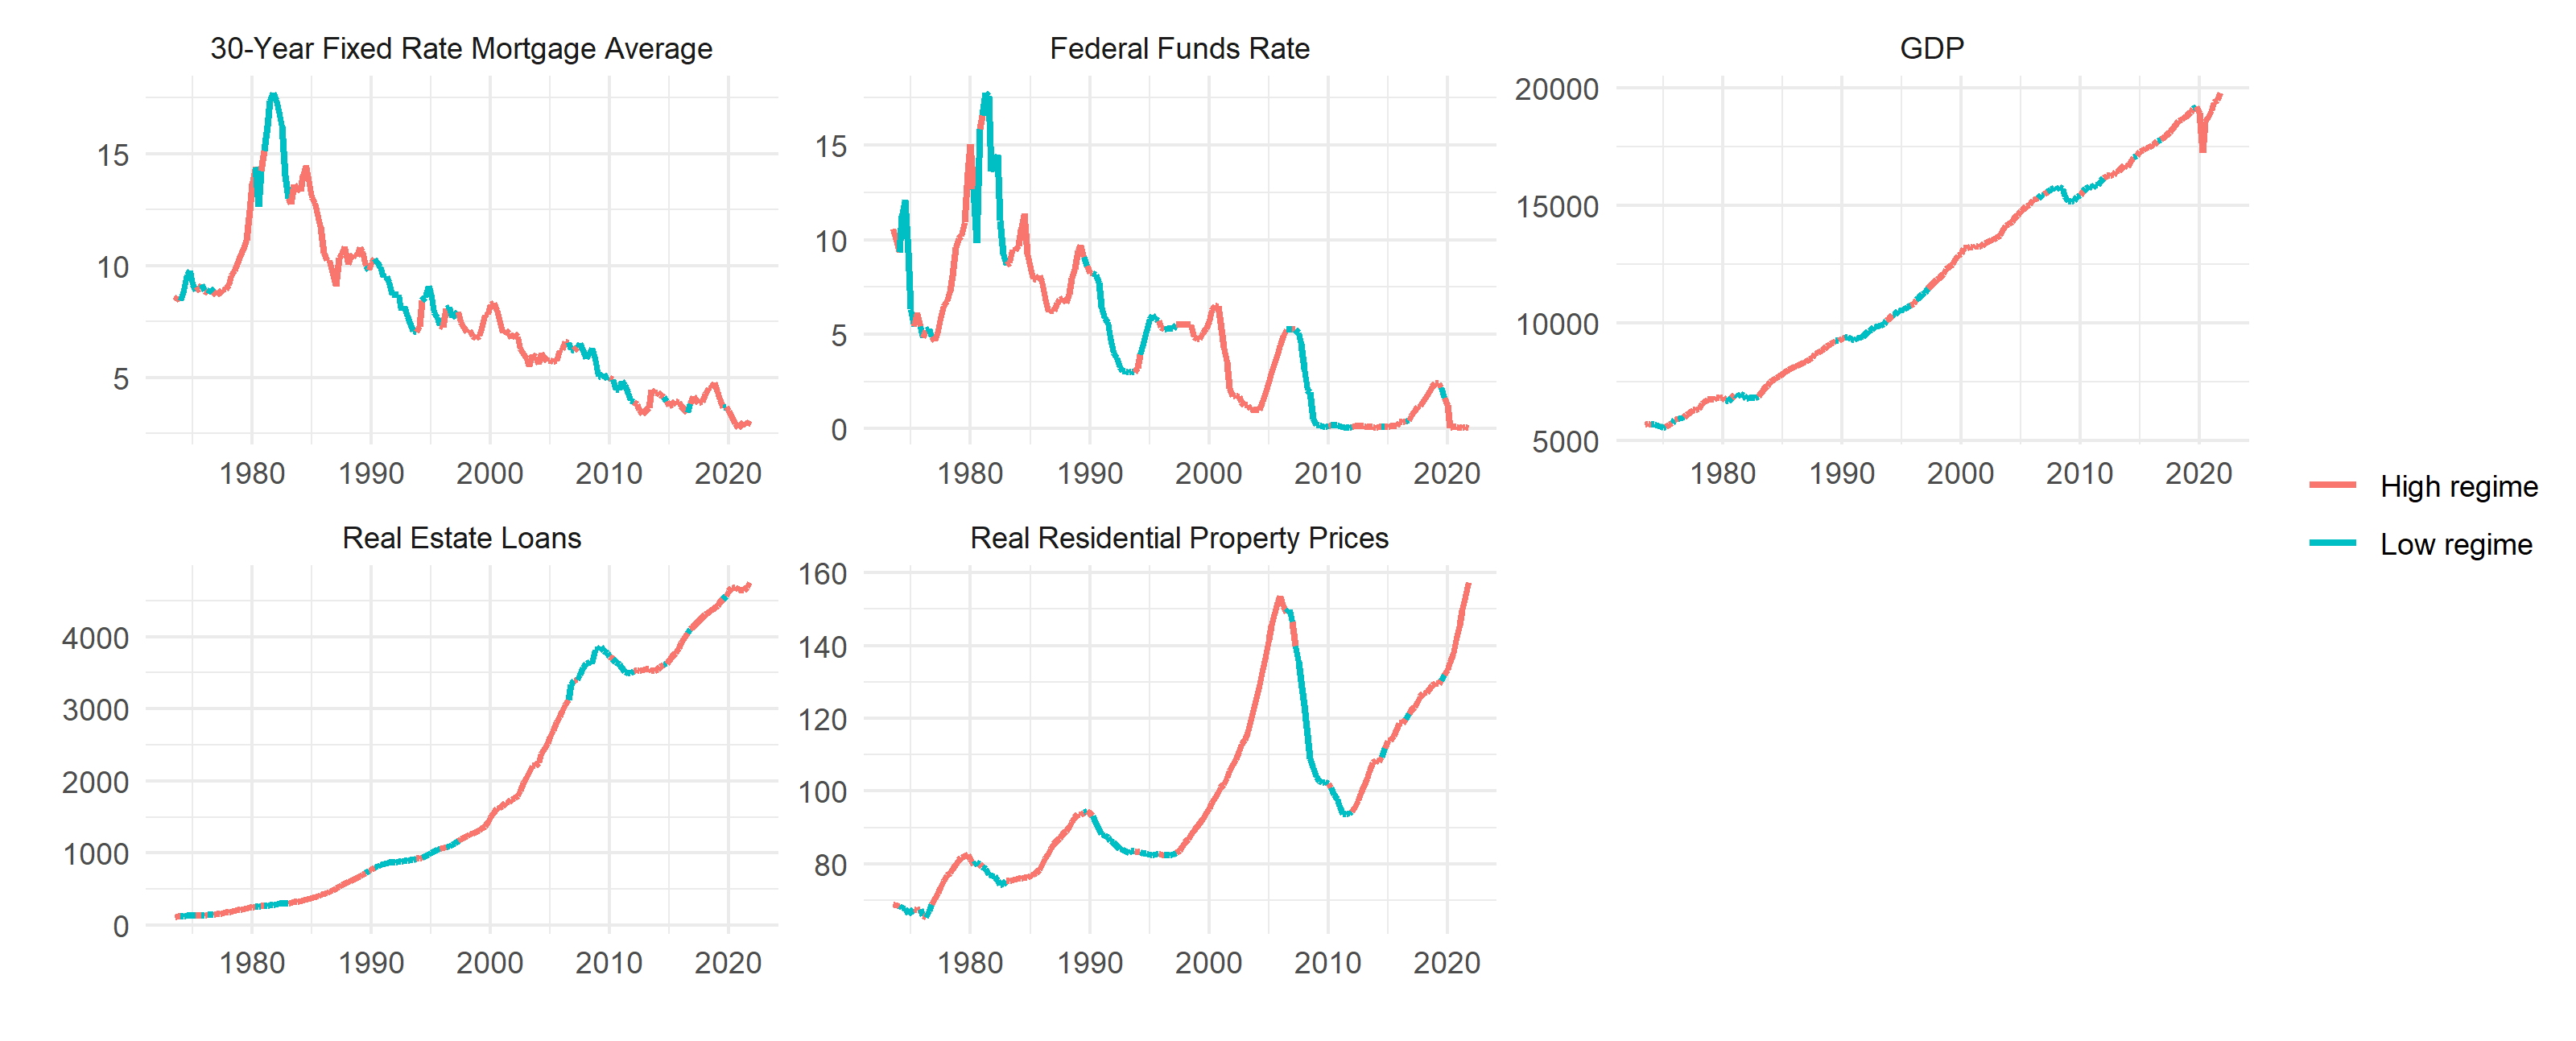
\includegraphics[width = \textwidth]{indicator.png}
		\caption{Time series plots of level variables with the regime indicator}
	\end{figure}
\end{center}
\noindent Here we can see that the indicator function's values - and thus the housing cycle -  do not always evidently coincide with the business cycle, however, there would likely be high correlation between a business cycle and a housing cycle indicator.\\

As in the above example with the simple SVAR model, I will evaluate results using impulse responses. When assessing threshold VARs, the use of generalized IRFs (GIRFs) / non-linear IRFS (NLIRFs) is a common practice, as a shock can cause the economy to shift from one regime to another. However, as I am primarily interested how economic dynamics differ in the two regimes estimated, I believe reporting simple linear IRFs should suffice for each regime. Exploring questions such as 'does the size of the shock matter?' could be explored with the GIRF method, however that is beyond the scope of this paper.\\

\noindent In figures 5. and 6. below, we can see the impulse responses of a structural shock from a 1 percentage point interest rate rise in the high and low regimes respectively.
 \begin{center}
	\begin{figure}[h!]
		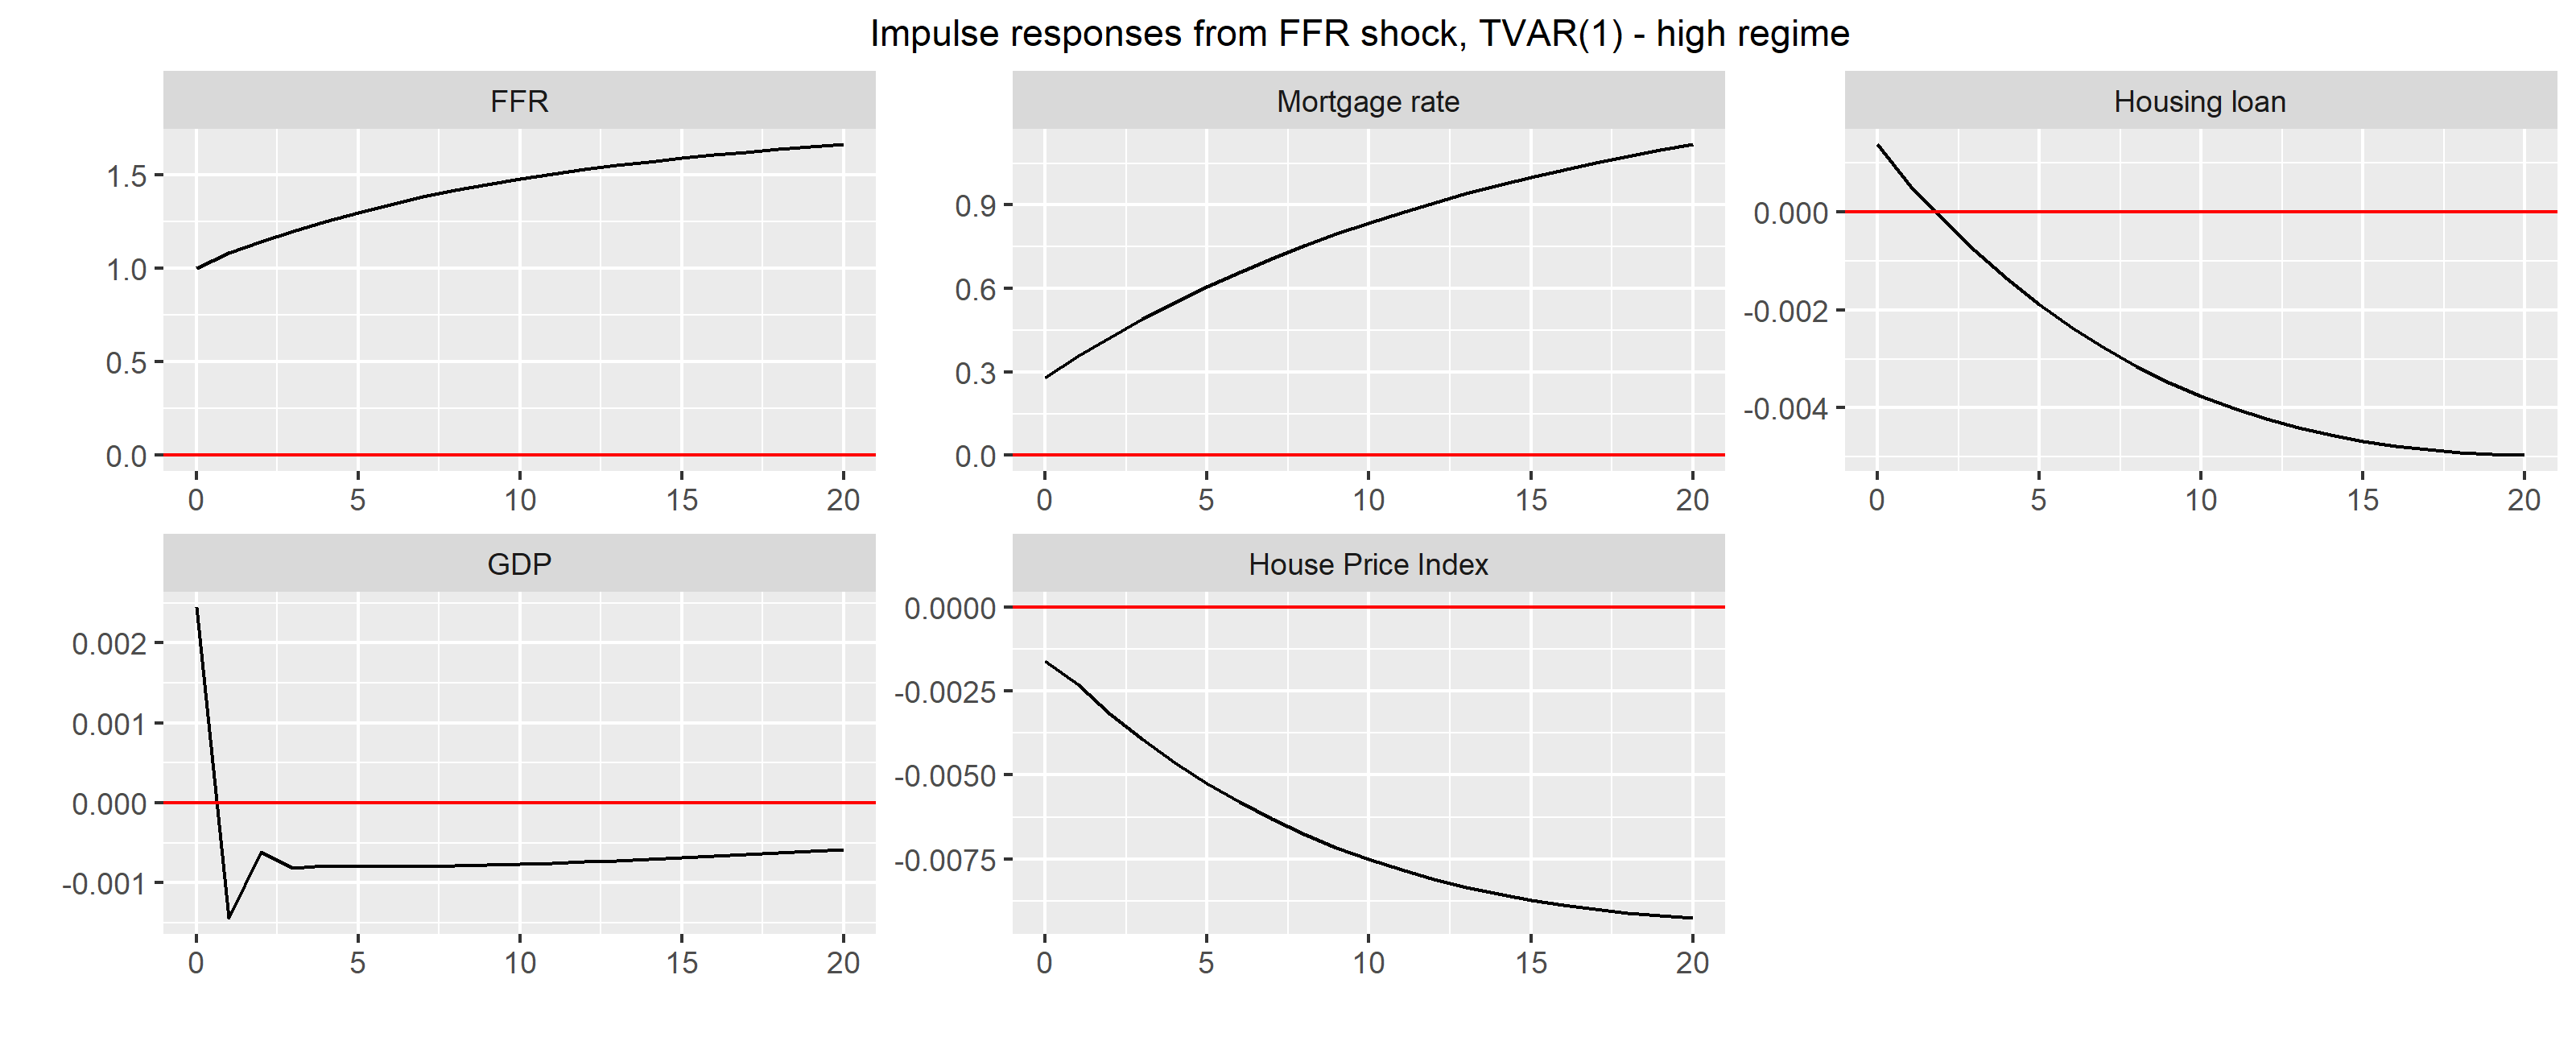
\includegraphics[width = \textwidth]{tvarhigh.png}
		\caption{Impulse responses of a 1 percentage point interest rate rise in TVAR(1) model - high regime}
	\end{figure}
\end{center}

 \begin{center}
	\begin{figure}[h!]
		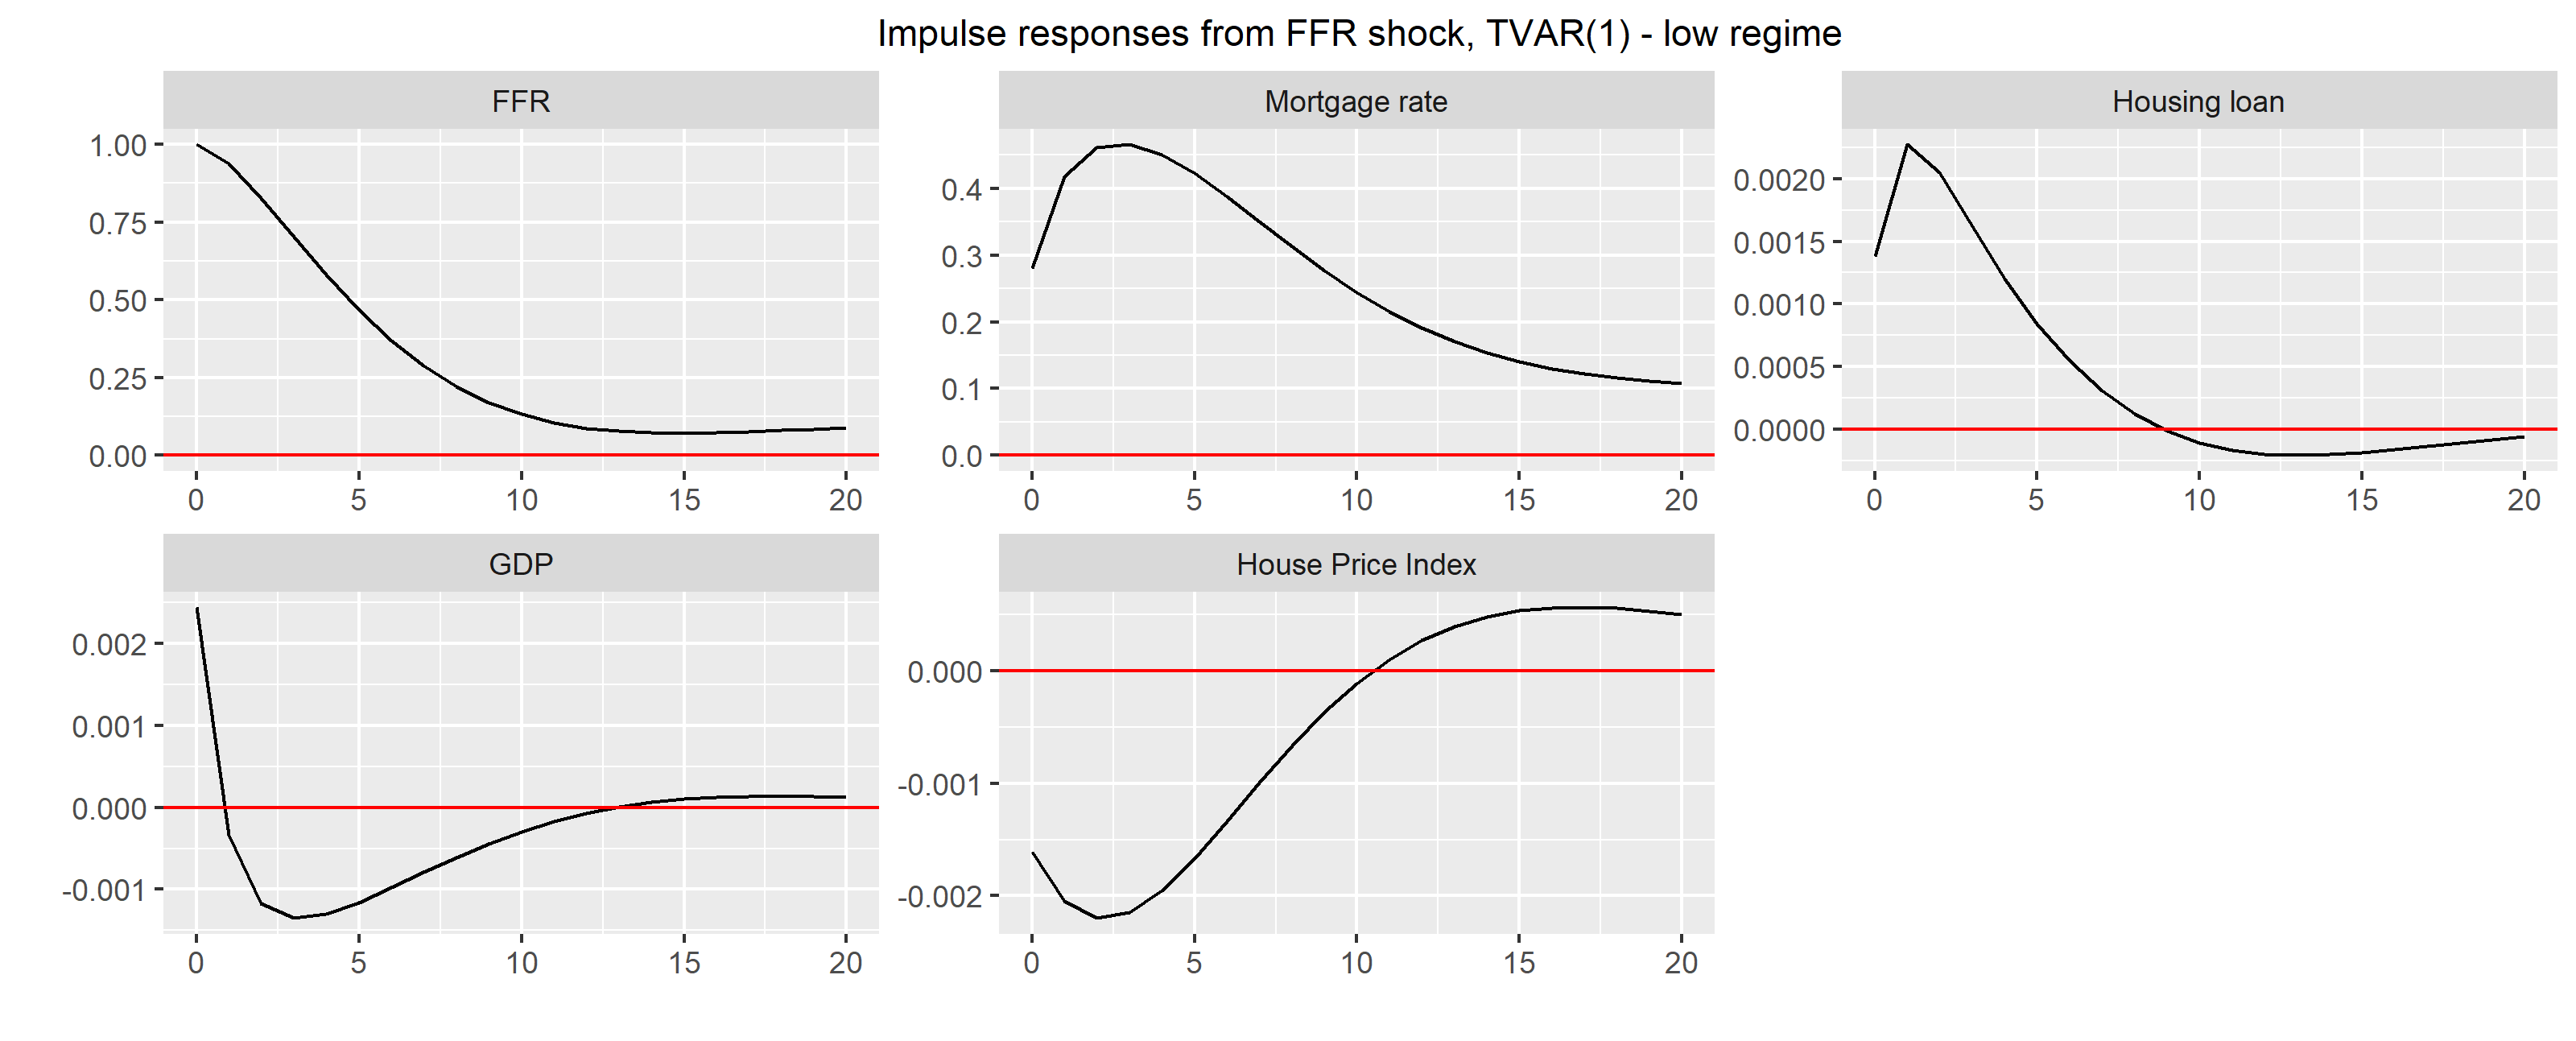
\includegraphics[width = \textwidth]{tvarlow.png}
		\caption{Impulse responses of a 1 percentage point interest rate rise in TVAR(1) model - low regime}
	\end{figure}
\end{center}
As we can see from the impulse responses above, the economic dynamics in the two regimes differ quite a bit. The FFR shock in the high regime shows extreme persistence compared to its low regime counterpart. This effect can also be seen in the 30-year mortgage average rate as well, with its more sluggish adjustment time.\\
\noindent In the responses of housing loan volume in the high regime, we see a minor rise, followed by a persistent drop. This can be explained by the drop in real estate prices incentivizing investors to purchase new properties, however, as the mortgage rate is persistently increasing, and prices continue to drop, the incentive turns into disincentive. Here we could say there is clear evidence for the credit channel of monetary policy. In the low regime, however we see that even though mortgage rates rise, so do housing loans. This could imply that there is a strong expectation of long run growth in housing prices thus expecting higher returns on real estate investments than the mortgage cost, especially as there only is a minor temporary drop in housing prices with a quick rebound, and that the interest rate shock is far less persistent. Thus in the low regime we can see that the credit channel is ineffective.\\
\noindent The response of economic activity seems somewhat similar to the simple SVAR model with a minor increase on impact and an economic contraction 1-2 quarters after the interest rate rise and thus a similar explanation can be given. An interesting outcome however is that this minor contraction in GDP growth is more persistent in the higher regime case, with no rebound to the steady state in sight.\\ 
And finally we see a relatively minor drop in housing prices in both regimes, however - likely as the interest rate shock is less persistent - in the low regime we see a quick rebound and the growth rate stabilizing just above 0 percentage point growth rate, whereas in the high regime housing prices continue to drop as the credit channel seems effective.\\

\noindent An interesting outcome to note is that if I were to extend the range beyond 20 quarters, while the low regime impulse responses seem to converge to a stable value, the high regime responses seem to explode. This would indicate that there is only one stable equilibrium in the model, which is in the low regime. With this in mind, we can say that there is empirical evidence that interest rate hikes can indeed burst the housing bubble.\\


\section{Conclusion}
In this paper I attempted to study the non-linear relationship between the housing market and the economy. I hypothesized that interest rate shocks hit the housing market much heavier, when the market is already heated. To study this non-linear relationship I fitted a two-regime TVAR model over some key economic variables from the US. I found strong empirical evidence regarding my hypothesis, even going as far as there not being a stable equilibrium of the housing market when it is in above its trend. A caveat to be mentioned although is that this empirical evidence - based on my analysis - is only true for the US. Different loan conditions could lead to different results, thus this paper should later be extended to find evidence from several countries. Future research possibilities could include replacing the TVAR model for a TVECM one to better understand the long-run relationship between the economy, monetary policy and the housing market.
 
\printbibliography[title = References]

\section*{Appendix}
Below can be seen the codes for replication (also attached in the Moodle submission platform).
The code is completely original, and easy to replicate (as all input is taken from the Federal Reserve Database directly, and the "folder" is only used to save the included plots - the code runs even if no alternative is given, and the error messages only affect the plot saving commands). For the modeling part I was primarily relying on the "tsDyn" package - containing the TVAR and associated LR test -  created by \cite{stigler2019}.
\begin{verbatim}
	#packages
	suppressPackageStartupMessages({
		library(readxl)
		library(tidyverse)
		library(tseries)
		library(forecast)
		library(TSA)
		library(aTSA)
		library(fpp2)
		library(lmtest)
		library(vars)
		library(mFilter)
		library(ggplot2)
		library(tsDyn)
		library(fredr)
		library(lubridate)
		library(cowplot)
		library(gridExtra)
		library(patchwork)
		library(data.table)
		library(tsibble)
		library(xts)
		library(zoo)
		library(broom)
		library(urca)
	})
	
	
	
	folder <- "C:/Users/horva/Documents/Egyetem/PhD/Study material/Semester 2/Time series/Empirical project"
	
	#set api key
	fredr_set_key("cda47ae66b38ed7988c0a9c2ec80c94f")
	
	#download data
	params <- list(
	series_id = c("QUSR628BIS", "RELACBW027SBOG", "MORTGAGE30US", "DFF", "GDPC1"),
	frequency = "q",
	observation_start = as.Date("1950-01-01")
	)
	
	
	import  <- pmap_dfr(
	.l = params,
	.f = ~ fredr(series_id = .x, frequency = .y)
	) %>%
	dplyr::select(date, series_id, value) %>%
	spread(key = series_id, value = value) %>%
	drop_na() %>% as_tsibble() %>% rename(ffr = DFF,
	m30 = MORTGAGE30US,
	hloan = RELACBW027SBOG,
	gdp = GDPC1,
	hprice = QUSR628BIS) %>%
	drop_na()
	
	import %>% as_tibble() %>% gather(key = "variable", value = "value", ffr, m30, hloan, gdp, hprice) %>%
	mutate(variable = case_when(variable == "ffr" ~ "Federal Funds Rate",
	variable == "gdp" ~ "GDP",
	variable == "hloan" ~ "Real Estate Loans",
	variable == "hprice" ~ "Real Residential Property Prices",
	variable == "m30" ~ "30-Year Fixed Rate Mortgage Average")) %>%
	ggplot(aes(x = date, y = value)) +
	geom_line() +
	facet_wrap(~variable, scales = "free") + theme_minimal() +
	labs(x = "",
	y = "") 
	ggsave(file.path(folder, "dataplot.png"),
	device = "png")
	
	
	data <- import %>% 
	mutate(hloan = log(hloan),
	gdp = log(gdp),
	hprice = log(hprice),
	hloan = hloan - lag(hloan),
	gdp = gdp - lag(gdp),
	hprice = hprice - lag(hprice)) %>%
	drop_na() %>%
	relocate(ffr, .after = date) %>%
	relocate(m30, .after = ffr) %>%
	relocate(hloan, .after = m30) %>%
	relocate(gdp, .after = hloan) %>%
	relocate(hprice, .after = gdp)
	
	
	#plotting log-differenced gdp, house price index and housing loand volume
	ggplot(data) +
	geom_line(aes(x = date, y = gdp), color = "blue") +
	geom_line(aes(x = date, y = hprice), color = "darkgreen") +
	geom_line(aes(x = date, y = hloan), color = "red") +
	theme_minimal() +
	theme(plot.title = element_text(size = 11, hjust=0.5),
	axis.title.y = element_text(size=11)) +
	labs(y = "",
	x = "Date",
	title = "GDP (blue), House Price Index (green) and Housing loan volume (red) for the US, log-difference")
	
	#cross correlations
	cor(data$gdp, data$hprice)
	cor(data$gdp, data$hloan)
	cor(data$hloan, data$hprice)
	
	data <- data[, 2:6] %>% ts()
	
	
	
	
	#fitting simple var model
	VARselect(data)
	
	var <- VAR(data, p = 1, type = "const")
	
	varcoef <- bind_rows(
	var$varresult$ffr$coefficients,
	var$varresult$m30$coefficients,
	var$varresult$hloan$coefficients,
	var$varresult$gdp$coefficients,
	var$varresult$hprice$coefficients) %>%
	as.matrix()
	
	#identify structural shocks
	e <- resid(var)
	cov_mat <- t(e) %*% e
	chol <- chol(cov_mat)
	
	print(chol) %>% t()
	
	ffrshock <- chol[1,] / chol[1,1]
	
	irfgen <- function(shock, nahead, coefmat, main){
		
		irf<- matrix(nrow = length(shock), ncol = nahead+1)
		irf[,1] <- shock %>% as.matrix()
		t <- matrix(ncol = 1, nrow = nahead+1)
		
		for(j in 1:ncol(irf)){
			t[j, 1] <- j-1
		}
		
		for(j in 2:ncol(irf)){
			for(i in 1:nrow(irf)){
				irf[i,j] <- irf[1,j-1]*coefmat[i,1]+
				irf[2,j-1]*coefmat[i,2]+
				irf[3,j-1]*coefmat[i,3]+
				irf[4,j-1]*coefmat[i,4]+
				irf[5,j-1]*coefmat[i,5]
			}
		}
		
		irf <- t(irf)
		
		colnames(irf) <- names(shock)
		irf <- bind_cols(t, irf) %>%
		as_tibble() %>%
		rename(t = ...1)
		
		irf <- gather(irf, key = "variable", value = "response", ffr, m30, hloan, gdp, hprice) %>%
		mutate(variable = case_when(variable == "ffr" ~ "FFR",
		variable == "m30" ~ "Mortgage rate",
		variable == "hloan" ~ "Housing loan",
		variable == "gdp" ~ "GDP",
		variable == "hprice" ~ "House Price Index"),
		variable = factor(variable, levels = c("FFR", "Mortgage rate", "Housing loan", "GDP", "House Price Index")))
		
		ggplot(irf, aes(x = t, y = response)) +
		geom_line() +
		geom_hline(yintercept = 0, color = "red")+
		facet_wrap(~variable, scales = "free") +
		labs(x = "",
		y = "",
		title = main)+
		theme(plot.title = element_text(size = 11, hjust=0.5),
		axis.title.y = element_text(size=11))
		
	}
	
	irfgen(shock = ffrshock,
	nahead = 20,
	coefmat = varcoef,
	main = "Impulse responses of FFR shock, simple SVAR(1)")
	ggsave(file.path(folder, "svarirf.png"),
	device = "png")
	
	#teszteljük a tvar helyességét
	par_orig <- c(5.1, 4.1, 4.1, 2.1)
	par_large <- c(2,2,2,2)
	par(mar = par_large)
	png(file.path(folder, "tvartest.png"))
	TVAR.LRtest(data, lag = 1, mTh = 5, plot = TRUE, nboot = 10000)
	dev.off()
	par(mar = par_orig)
	
	#tvar with optimal threshold value - possibly not very useful
	tvar <- TVAR(data, lag = 1, nthresh = 1, mTh = 5, model = "TAR", max.iter = 1000, trim = 0)  
	print(tvar)
	summary(tvar)
	plot(tvar)
	
	#tvar with threshold value = 0 - a compromised solution
	tvar <- TVAR(data, lag = 1, nthresh = 1, mTh = 5, model = "TAR", max.iter = 1000, gamma = 0)  
	print(tvar)
	summary(tvar)
	plot(tvar)
	
	#identify structural shocks
	e <- resid(tvar)
	cov_mat <- t(e) %*% e
	chol <- chol(cov_mat)
	
	print(chol) %>% t()
	
	ffrshock <- chol[1,] / chol[1,1]
	
	highcoef <- tvar$coefficients$Bup
	
	lowcoef <- tvar$coefficients$Bdown
	
	irfgen <- function(shock, nahead, coefmat, main){
		
		irf<- matrix(nrow = length(shock), ncol = nahead+1)
		irf[,1] <- shock %>% as.matrix()
		t <- matrix(ncol = 1, nrow = nahead+1)
		
		for(j in 1:ncol(irf)){
			t[j, 1] <- j-1
		}
		
		for(j in 2:ncol(irf)){
			for(i in 1:nrow(irf)){
				irf[i,j] <- irf[1,j-1]*coefmat[i,2]+
				irf[2,j-1]*coefmat[i,3]+
				irf[3,j-1]*coefmat[i,4]+
				irf[4,j-1]*coefmat[i,5]+
				irf[5,j-1]*coefmat[i,6]
			}
		}
		
		irf <- t(irf)
		
		colnames(irf) <- names(shock)
		irf <- bind_cols(t, irf) %>%
		as_tibble() %>%
		rename(t = ...1)
		
		irf <- gather(irf, key = "variable", value = "response", ffr, m30, hloan, gdp, hprice) %>%
		mutate(variable = case_when(variable == "ffr" ~ "FFR",
		variable == "m30" ~ "Mortgage rate",
		variable == "hloan" ~ "Housing loan",
		variable == "gdp" ~ "GDP",
		variable == "hprice" ~ "House Price Index"),
		variable = factor(variable, levels = c("FFR", "Mortgage rate", "Housing loan", "GDP", "House Price Index")))
		
		ggplot(irf, aes(x = t, y = response)) +
		geom_line() +
		geom_hline(yintercept = 0, color = "red")+
		facet_wrap(~variable, scales = "free")+
		labs(x = "",
		y = "",
		title = main)+
		theme(plot.title = element_text(size = 11, hjust=0.5),
		axis.title.y = element_text(size=11))
		
		
	}
	
	
	irfgen(shock = ffrshock,
	nahead = 20,
	coefmat = highcoef,
	main = "Impulse responses from FFR shock, TVAR(1) - high regime")
	ggsave(file.path(folder, "tvarhigh.png"),
	device = "png")
	
	irfgen(shock = ffrshock,
	nahead = 20,
	coefmat = lowcoef,
	main = "Impulse responses from FFR shock, TVAR(1) - low regime")
	ggsave(file.path(folder, "tvarlow.png"),
	device = "png")
	
	indicator <- tvar$model.specific$regime
	
	import %>% filter(date >= as.Date("1973-04-01")) %>%
	bind_cols(indicator) %>%
	drop_na() %>%
	rename(indicator = ...7) %>%
	as_tibble() %>% gather(key = "variable", value = "value", ffr, m30, hloan, gdp, hprice) %>%
	mutate(variable = case_when(variable == "ffr" ~ "Federal Funds Rate",
	variable == "gdp" ~ "GDP",
	variable == "hloan" ~ "Real Estate Loans",
	variable == "hprice" ~ "Real Residential Property Prices",
	variable == "m30" ~ "30-Year Fixed Rate Mortgage Average")) %>%
	mutate(indicator = case_when(indicator == 1 ~ "Low regime",
	indicator == 2 ~ "High regime")) %>%
	ggplot(aes(x = date, y = value, color = indicator, group = 1)) +
	geom_line(size = 1) +
	facet_wrap(~variable, scales = "free") + theme_minimal() +
	labs(x = "",
	y = "") +
	theme(legend.title = element_blank()) 
	ggsave(file.path(folder, "indicator.png"),
	device = "png")
	
	
\end{verbatim}

\end{document}